\documentclass[11pt]{article}

% ==== Paquetes ====
\usepackage[utf8]{inputenc}
\usepackage[spanish]{babel}
\usepackage{amsmath, amssymb, amsfonts, siunitx}
\usepackage{graphicx}
\usepackage{float}
\usepackage{listings} % Para código
\usepackage{pdfpages}
\usepackage{xcolor}
\usepackage{hyperref}
\usepackage{caption}
\usepackage{subcaption}
\usepackage{geometry}
\usepackage{tikz}

\geometry{margin=2.5cm}

% ==== Configuración de listings (para código) ====
\lstset{
  basicstyle=\ttfamily\small,
  numbers=left,
  numberstyle=\tiny,
  stepnumber=1,
  numbersep=5pt,
  backgroundcolor=\color{gray!10},
  frame=single,
  tabsize=2,
  breaklines=true,
  showstringspaces=false,
  keywordstyle=\color{blue},
  commentstyle=\color{green!50!black},
  stringstyle=\color{red!70!black},
  literate={á}{{\'a}}1 {é}{{\'e}}1 {í}{{\'i}}1
           {ó}{{\'o}}1 {ú}{{\'u}}1 {ñ}{{\~n}}1
           {Á}{{\'A}}1 {É}{{\'E}}1 {Í}{{\'I}}1
           {Ó}{{\'O}}1 {Ú}{{\'U}}1 {Ñ}{{\~N}}1
}

% ==== Datos de la tarea ====
\title{IEE3584 - Procesamiento Avanzado de Señales \\
Tarea 4}
\author{Nicolás Seguel}
\date{Septiembre 2025}

\begin{document}

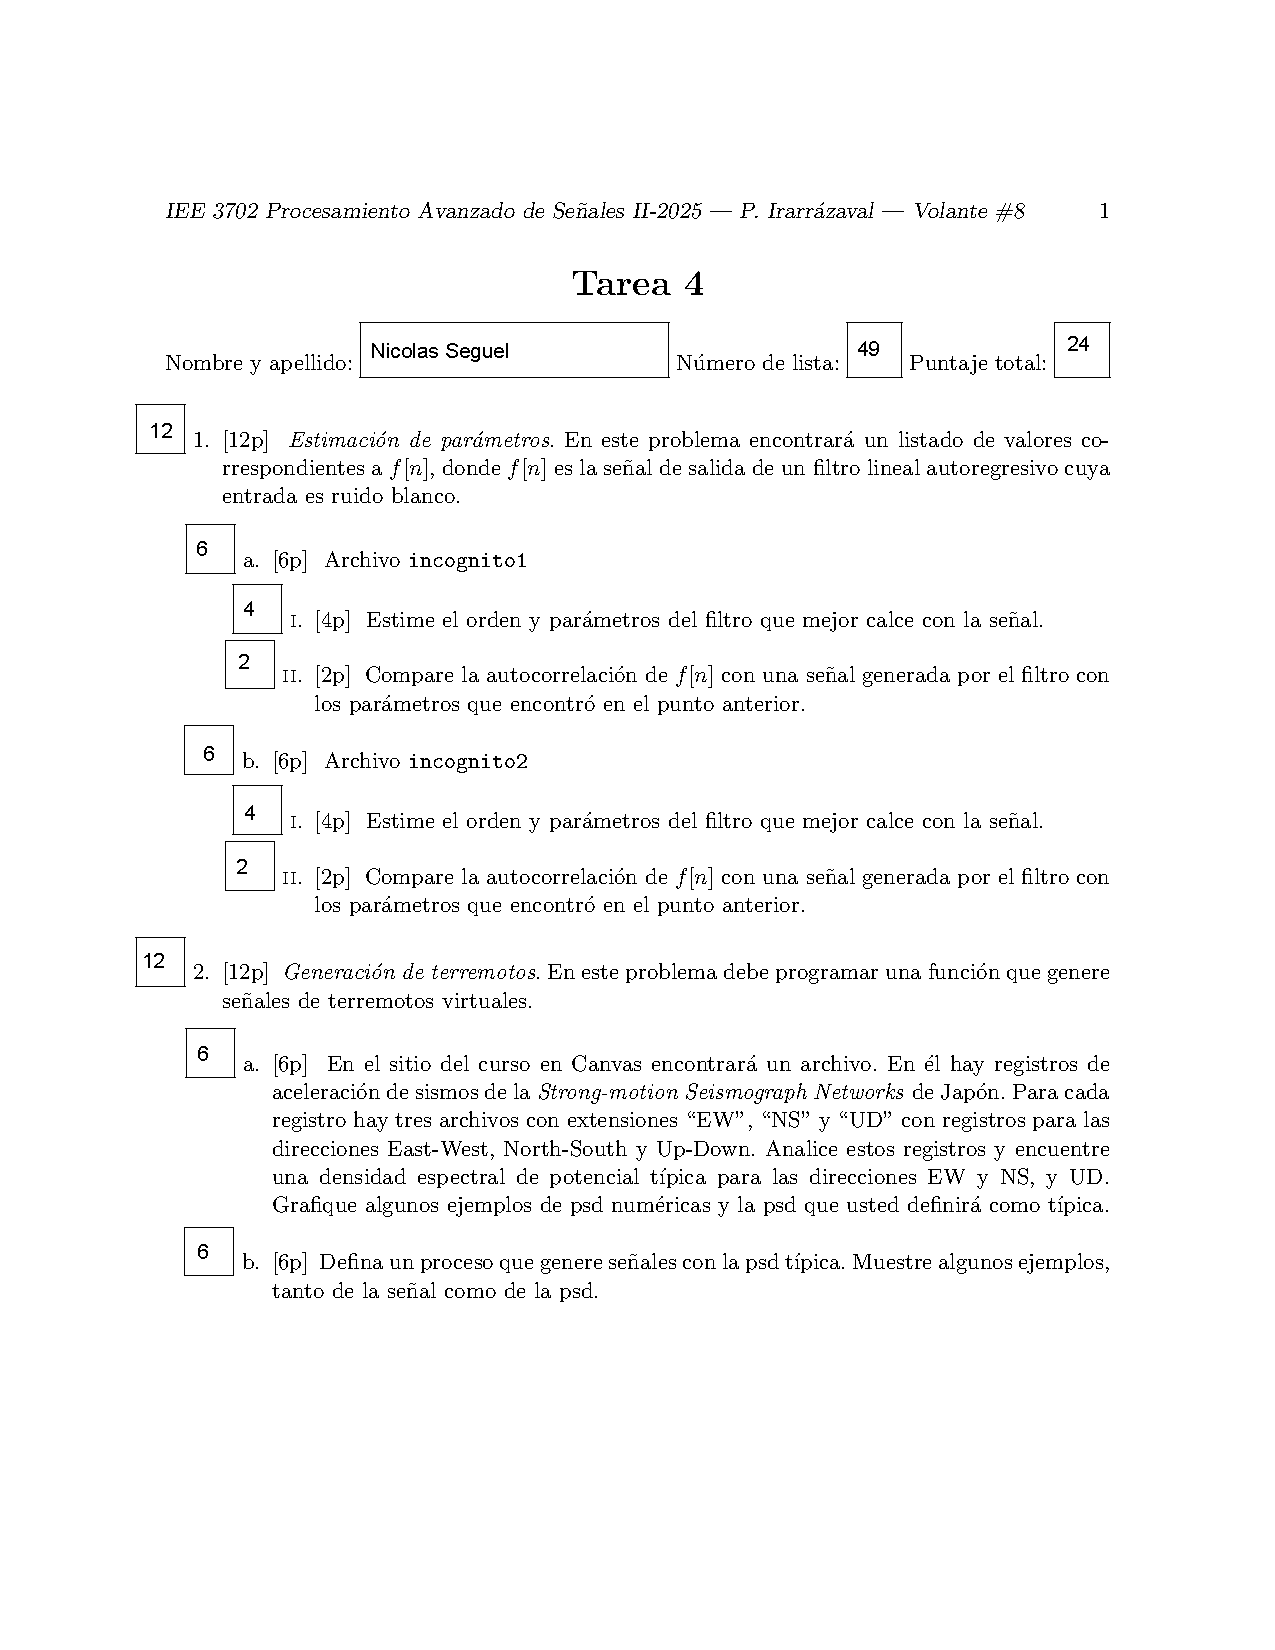
\includepdf[pages=-]{08.tarea04.pdf}
\maketitle

% ==== Problema 1 ====
% ==== Problema 1 ====
\section{Problema 1}

\subsection{incognito1}

\subsubsection{Estimación}

Se estimó el orden del modelo AR utilizando el criterio de información de Akaike (AIC). 
En la Figura~\ref{fig:aic1} se muestra la evolución del AIC en función del orden, donde 
se observa un mínimo en $p=22$. 

\begin{figure}[H]
    \centering
    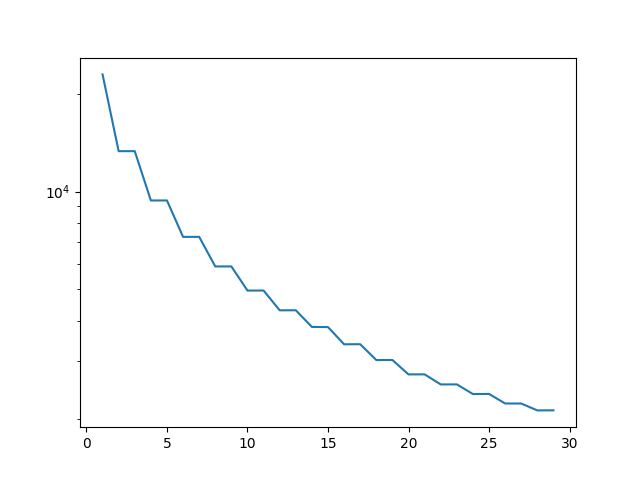
\includegraphics[width=0.7\textwidth]{AIC_order_estimation_1.png}
    \caption{Estimación del orden AR usando AIC para \texttt{incognito1}.}
    \label{fig:aic1}
\end{figure}

Los coeficientes estimados del filtro AR(22) y la varianza del ruido fueron:

\[
\text{Coeficientes AR} = 
\begin{bmatrix}
-0.0056 & 0.9270 & -0.0078 & 0.8438 & -0.0115 & 0.7588 & -0.0172 & 0.6740 \\
-0.0204 & 0.5873 & -0.0140 & 0.5029 & -0.0171 & 0.4218 & -0.0195 & 0.3426 \\
-0.0047 & 0.2543 & -0.0016 & 0.1649 & 0.0052 & 0.0762
\end{bmatrix}
\]

\[
\sigma^2 = 1.0794
\]

\subsubsection{Autocorrelación}

En la Figura~\ref{fig:autocorr1} se comparan las autocorrelaciones de la señal original 
y de la señal generada con el modelo estimado. Se observa que el modelo captura 
adecuadamente la estructura de la autocorrelación, en particular la anulación de los 
retardos impares y la similitud en los retardos pares.

\begin{figure}[H]
    \centering
    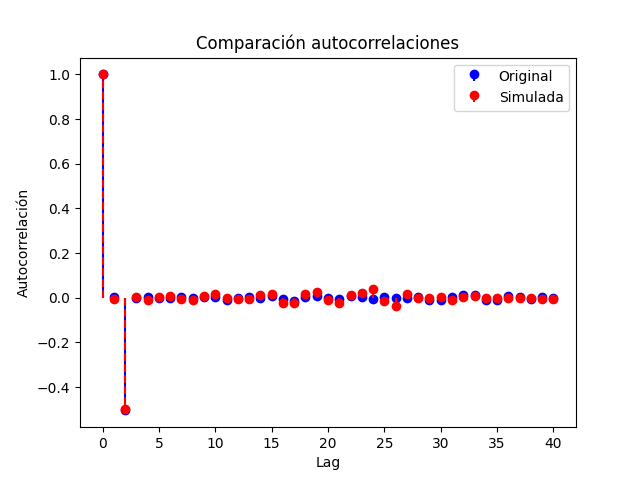
\includegraphics[width=0.7\textwidth]{AutoCorr_1.png}
    \caption{Comparación de autocorrelaciones para \texttt{incognito1}.}
    \label{fig:autocorr1}
\end{figure}

% ---------------------------

\subsection{incognito2}

\subsubsection{Estimación}

Para este caso, la Figura~\ref{fig:aic2} muestra el criterio AIC en función del orden. 
El mínimo se encontró en $p=4$.

\begin{figure}[H]
    \centering
    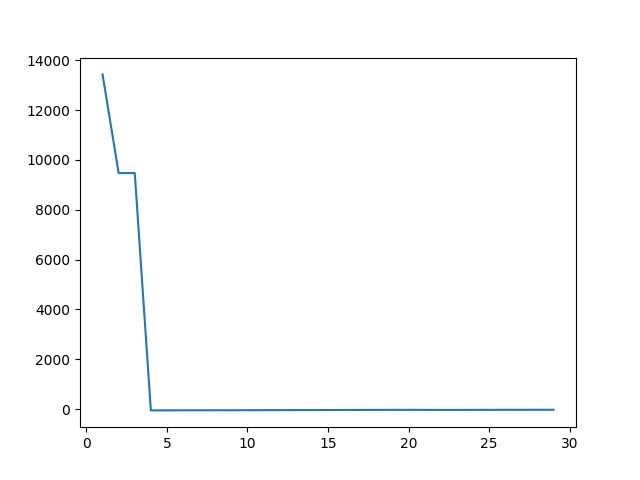
\includegraphics[width=0.7\textwidth]{AIC_order_estimation_2.png}
    \caption{Estimación del orden AR usando AIC para \texttt{incognito2}.}
    \label{fig:aic2}
\end{figure}

Los parámetros estimados del modelo AR(4) son:

\[
\text{Coeficientes AR} = 
\begin{bmatrix}
-0.0051 & 0.5071 & -0.0014 & 0.5023
\end{bmatrix}
\]

\[
\sigma^2 = 0.9980
\]

\subsubsection{Autocorrelación}

En la Figura~\ref{fig:autocorr2} se comparan las autocorrelaciones de la señal original 
y de la señal generada. Se aprecia que el modelo de orden 4 logra reproducir la 
estructura estadística de la señal.

\begin{figure}[H]
    \centering
    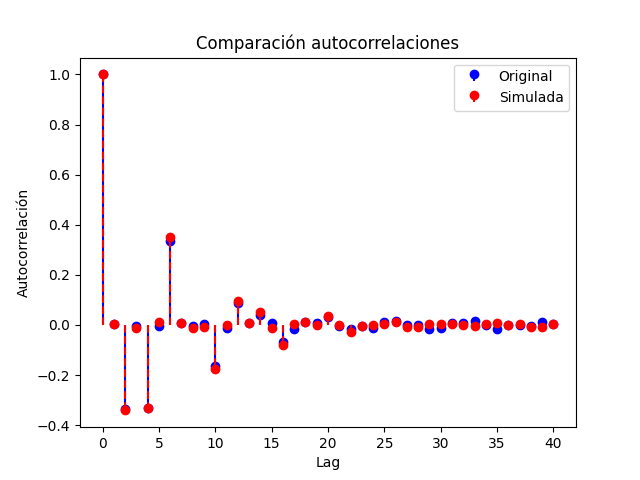
\includegraphics[width=0.7\textwidth]{AutoCorr_2.png}
    \caption{Comparación de autocorrelaciones para \texttt{incognito2}.}
    \label{fig:autocorr2}
\end{figure}


% ==== Problema 2 ====
\section{Problema 2}

\subsection{Densidad espectral de potencia de un sismo}

Se analizaron registros de aceleración de sismos en las tres direcciones (East-West, North-South y Up-Down).  
Para cada archivo se estimó la densidad espectral de potencia (PSD) utilizando el método de Welch, y se definió como PSD típica el promedio de todas las PSD obtenidas en cada dirección.  

A continuación se muestran ejemplos de PSD individuales junto con la PSD típica en cada componente:

\begin{figure}[H]
    \centering
    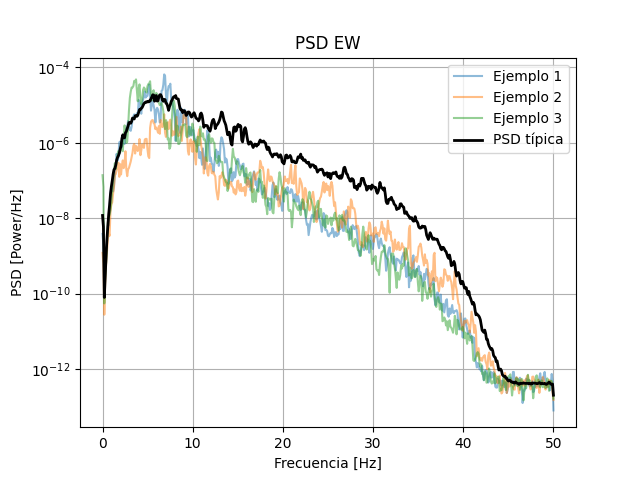
\includegraphics[width=0.7\textwidth]{PSD_EW.png}
    \caption{Ejemplos de PSD y PSD típica en dirección East-West.}
    \label{fig:psd_ew}
\end{figure}

\begin{figure}[H]
    \centering
    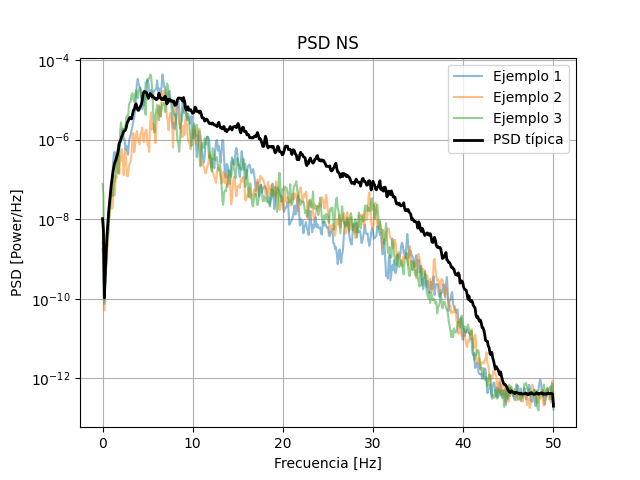
\includegraphics[width=0.7\textwidth]{PSD_NS.png}
    \caption{Ejemplos de PSD y PSD típica en dirección North-South.}
    \label{fig:psd_ns}
\end{figure}

\begin{figure}[H]
    \centering
    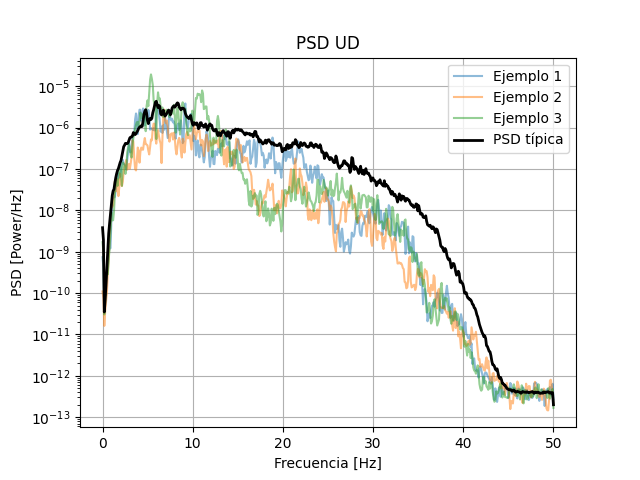
\includegraphics[width=0.7\textwidth]{PSD_UD.png}
    \caption{Ejemplos de PSD y PSD típica en dirección Up-Down.}
    \label{fig:psd_ud}
\end{figure}

\subsection{Generación de señales de sismos}

A partir de la PSD típica estimada para cada dirección, se generaron sismos virtuales mediante el método de filtrado espectral:  
se construyó un espectro con magnitud $\sqrt{\text{PSD}(f)}$ y fase aleatoria, y se aplicó transformada inversa de Fourier para obtener la señal en el dominio del tiempo.  

En las siguientes figuras se muestran ejemplos de terremotos sintéticos y la comparación entre la PSD típica y la PSD de la señal generada:

\begin{figure}[H]
    \centering
    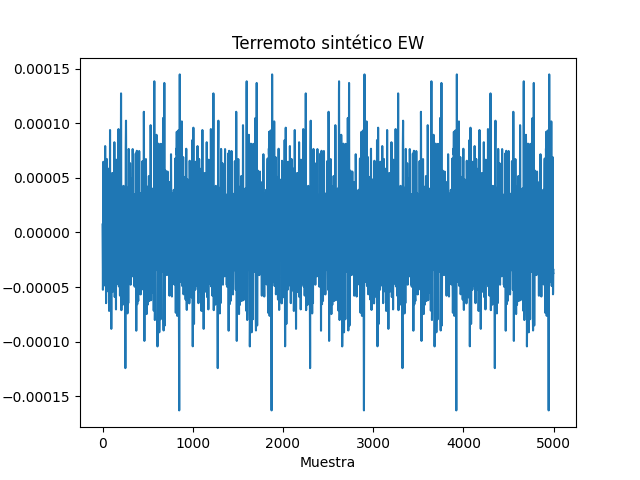
\includegraphics[width=0.7\textwidth]{SismoSintetico_EW.png}
    \caption{Ejemplo de terremoto sintético en dirección East-West.}
    \label{fig:sismo_ew}
\end{figure}

\begin{figure}[H]
    \centering
    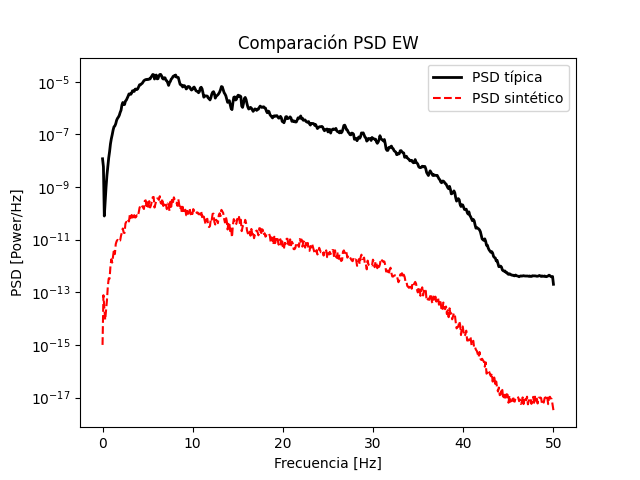
\includegraphics[width=0.7\textwidth]{PSD_comparacion_EW.png}
    \caption{Comparación entre PSD típica y PSD de terremoto sintético en dirección East-West.}
    \label{fig:psdcomp_ew}
\end{figure}

\begin{figure}[H]
    \centering
    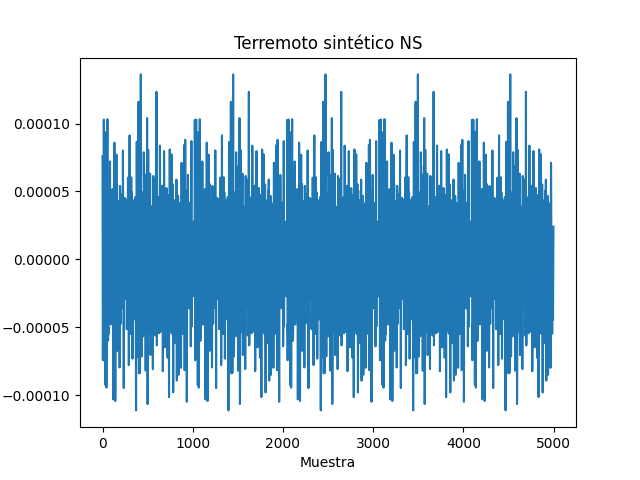
\includegraphics[width=0.7\textwidth]{SismoSintetico_NS.png}
    \caption{Ejemplo de terremoto sintético en dirección North-South.}
    \label{fig:sismo_ns}
\end{figure}

\begin{figure}[H]
    \centering
    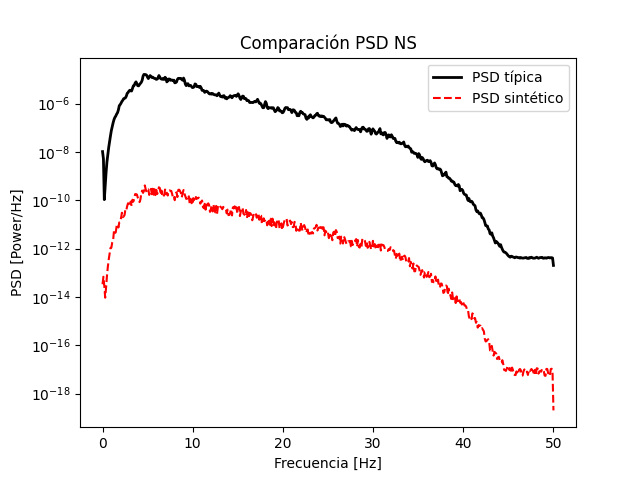
\includegraphics[width=0.7\textwidth]{PSD_comparacion_NS.png}
    \caption{Comparación entre PSD típica y PSD de terremoto sintético en dirección North-South.}
    \label{fig:psdcomp_ns}
\end{figure}

\begin{figure}[H]
    \centering
    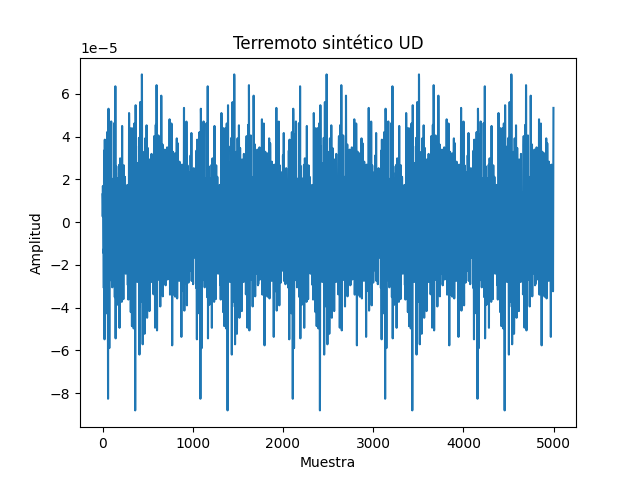
\includegraphics[width=0.7\textwidth]{SismoSintetico_UD.png}
    \caption{Ejemplo de terremoto sintético en dirección Up-Down.}
    \label{fig:sismo_ud}
\end{figure}

\begin{figure}[H]
    \centering
    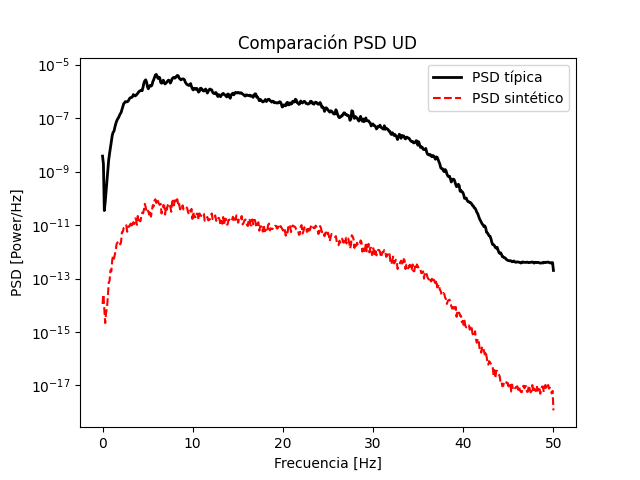
\includegraphics[width=0.7\textwidth]{PSD_comparacion_UD.png}
    \caption{Comparación entre PSD típica y PSD de terremoto sintético en dirección Up-Down.}
    \label{fig:psdcomp_ud}
\end{figure}

% ==== Anexo ====
\newpage
\appendix
\section*{Anexo: Códigos fuente}

A continuación se incluyen los códigos desarrollados en Python para la resolución de la tarea.

\subsection*{pregunta1.py}
\lstinputlisting[language=Python]{src/pregunta1.py}

\subsection*{pregunta2.py}
\lstinputlisting[language=Python]{src/pregunta2.py}


\end{document}
